\section{Evaluation}
\label{sec:eval}
We now evaluate the effectiveness of our processor and memory system optimizations for DNN training.  We conduct our evaluations along $3$ dimensions: (i) the impact on single thread performance (\ref{subsec:perf_single_thread}), (ii) the impact on multi-threading scalability in a server (\ref{subsec:perf_multi_thread}), and (iii)  the impact on model parallelism performance (\ref{subsec:perf_model_parallel}).  

 \subsection{Methodology}
 \label{subsec:eval_method}
 
 \paragraph{Real-world Image Recognition Workloads:} We used image recognition workloads to evaluate the impact of our optimizations on DNN training performance.  Image recognition models cover an important class of challenging AI problems, and training them to reasonable task accuracy requires copious amounts of compute and memory cycles~\cite{Krizhevsky12, Le12, Dean12, Chilimbi14}.  We used four real-world image recognition benchmarks in our experiments: (i) {\it MNIST}~\cite{Lecun98}, (ii) {\it CIFAR-10}~\cite{KrizhevskyThesis}, (iii) {\it ImageNet-1K}~\cite{imagenet09}, and (iv) {\it ImageNet-22K}~\cite{imagenet09}.  For our experiments, we replicate the architectures of a high quality (or the best performing) model for each task based on  prior work.  

\begin{itemize}
\item MNIST~\cite{Chilimbi14}: The task is the classification of $28$x$28$ grayscale images of handwritten digits into $10$ categories (i.e., $0$---$9$).  The model for this task is relatively small, containing about $2.5$ million in five layers.  

\item CIFAR-10~\cite{Srivastava14a}: The task is the classification of $32$x$32$ color images into $10$ categories. The model for learning this task is moderately large, containing $28.5$ million connections in five layers.

\item ImageNet-1K~\cite{Krizhevsky12} \& ImageNet-22K~\cite{Chilimbi14}: The tasks are the classification of $256$x$256$ color images into $1000$ and $22000$ categories respectively. The ImageNet-1K model is quite large and contains about $65$ million connections in seven layers.  The ImageNet-22K model is one of the largest image models available, and contains about $2$ billion connections in $8$ layers. 

\end{itemize} 

\paragraph{Experimental Approach}
We evaluate the performance of our optimizations using a combination of real and simulated hardware experiments.  We evaluate our computation sparsity optimizations on real hardware by hand-optimizing the loops in training kernels, for computation sparsity, as would be done by our proposed processor extensions.   And in our experiments we alternate execution of a loop and its sparsity-optimized version(s) based on computation and data sparsity information of the model (Section~\ref{subsec:sparsity_profile}).  Our experimental system is a dual-socket Intel Xeon E2450 CPU, with each socket having eight cores on running at 2.1 Ghz.  The memory system comprises of private $32$ KB L$1$ cache, private $256$  L$2$ cache, and a $20$MB shared L$3$ cache on each socket.    We evaluate our data sparsity optimizations in a simulation environment by prototyping our proposed zero-cache extensions in the GEM5 simulator~\cite{Binkert11}.  Table~\ref{tab:sim_parameters}  presents the simulation parameters.

\begin{table}[h]
\centering
\begin{tabular}{|l|c|}
\hline 
\multicolumn{2} {|c|} {GEM5 Simulator}  \\
\hline
Cache line size & 64 bytes \\ \hline
L1 (private) & 32KB \\ \hline
L2 (private) & 256KB \\ \hline
L3 (shared) &  20MB \\  \hline
Coherence protocol & MESI \\ \hline
Memory system & Ruby \\ \hline
RAM size & 4GB \\  
\hline 

\end{tabular}
\caption{Memory simulation parameters}
\label{tab:sim_parameters}
\end{table}

\paragraph{DNN Execution Framework} We measure DNN training performance in our experiments by executing the models in a framework that estimates the performance and scalability of DNN training~\cite{Yan15}.  The tool is basically a stripped-down version of full-featured training frameworks, such as CAFFE~\cite{jia2014caffe} and Adam~\cite{Chilimbi14}, that implements only the performance-critical steps of training: feed-forward evaluation, back-propagation, and weight updates.   The tool also supports thread parallelism and model parallelism in DNN training.  The lighweight nature of the tool makes it convenient to use for performance studies.  We adapted the tool for our work by extending it to synthesize sparse input data for each processing step based on the sparsity information that we collected from profiling actual training runs (as described in Section~\ref{subsec:data_sparsity}). 

\paragraph{Comparison to Software Approaches}
We compare our hardware approach to two software approaches: (i) a baseline approach that (SIMD) vectorizes and unrolls the loops in training kernels~\cite{Vanhoucke11}, and (ii) a software optimization of the baseline that exploits sparsity to dynamically check training data for zeroes in order to skip multiply and addition operations (Section~\ref{subsec:sparse_code_oppor}).  We heavily optimize this software approach to mitigate overheads of dynamic checks by applying the optimization only in situations that can yield significant benefits (e.g., skipping inner loop execution).  Consequently, we use {\it SW-SparseOpt} only for back-propagation and weight updates, but not feed-forward evaluation, after empirically verifying that this was the optimal decision.  In our results, we refer to the baseline, software-optimized, and hardware-optimized approaches as \emph{LoopUnrolling}, and \emph{SW-SparseOpt}, and \emph{HW-SparseOpt} respectively. 

%This software approach is more effective for training than sparse representations of matrices and/or vectors~\cite{IntelSparseMatrix}, because sparse representations are only efficient in situations where: (i) the input data is significantly sparse (i.e., $>95\%$), and (ii) the sparse input data is static such that the cost of sparse representation is armotized over many uses.   


\begin{comment}
 %Although we expect our optimizatons to be effective in general for training with gradient descent methods, we focus on image recognition because it represents an important class of AI problems for which significant accuracy improvements have being achieved through gradient descent training. Specifically, we measure the impact of our optimizations on the training of high quality DNN models on $3$ common image recognition workloads: (i) {\it MNIST}~\cite{Lecun98}, (ii) {\it CIFAR-10}~\cite{KrizhevskyThesis}, and (iii) {\it ImageNet}~\cite{imagenet09}. We describe each benchmark and correspodinging DNN in more details below. 

\begin{itemize}
\item \textbf{MNIST:} The task is to classify $28$x$28$ grayscale images of handwritten digits into $10$ categories. The DNN is relatively small, containing about $2.5$ million connections in $5$ layers: $2$ convolutional layers with pooling, $2$ fully connected layers, and a $10$-way output layer~\cite{Chilimbi14}.

\item \textbf{CIFAR-10:} The task is to classify $32$x$32$ color images into $10$ categories.  The DNN is moderately-sized, containing about $28.5$ million connections in $5$  layers: $2$ convolutional layers with pooling, $2$ fully connected layers, and a $10$-way output layer~\cite{Krizhevsky12}.

\item ImageNet:  The task is to classify $256$x$256$ color images from  a dataset of about $15$ million images into a number of categories.  We used the two standard versions of this benchmark: (i) classifying $1.2$ million images into $1000$ categories (a.k.a., {\it ImageNet-1K}), and (ii) classifying the entire data set into $22000$ categories (a.k.a. {\it ImageNet-22K}. We used the largest ImageNet task (i.e., {\it ImageNet-22K}), which is to classify $256$x$256$ color images into $22,000$ categories.  This DNN is extremely large, containing over $2$ billion connections in $8$ layers: $5$ convolutional layers with pooling, $2$ linear layers, and a $22,000$-way output layer~\cite{Chilimbi14}. 
\end{itemize}

 \paragraph{Comparison to Software Approach:}
 We compare our approach to a software optimization that dynamically checks training data for zeroes in order to skip multiply and addition operations (\ref{subsec:sparse_code_oppor}).  This software approach is more effective for training than using sparse representations of matrices and/or vectors~\cite{IntelSparseMatrix} due to the dynamic nature of data sparsity in training.  To mitigate the software check overheads, we apply this optimization only it situations that can yield significant benefits (e.g., skip inner loop execution). 

\paragraph{Simulation-based Approach:} 
We conduct our performance experiments in a simulation enviroment, which allows us to easily prototype our proposed memory system extensions (Section~\ref{sec:design}).  We use a modified version of Memsim~\cite{memsim,eaf}, a multi-core simulator that models out-of-order cores coupled with a DDR3-1066~\cite{ddr3} DRAM  simulator. All systems use a three-level cache hierarchy with a  uniform 64B cache line size. We do not enforce inclusion in any level of the hierarchy. We use the state-of-the-art DRRIP cache replacement policy~\cite{rrip} for the last-level cache. All our evaluated systems use an aggressive multi-stream  prefetcher~\cite{fdp} similar to the one implemented in IBM Power~6~\cite{power6-prefetcher}.


\end{comment}


           

   
\subsection{Computation Sparsity Optimizations}
\label{subsec:perf_computation_sparsity}
Computation sparsity optimizations improve DNN training performance by dynamically skipping execution on zero data values.  We measure the impact of our computation sparsity optimizations on a single-threaded training and multi-threaded training. 

\subsubsection{Single-Threaded Performance}
Figure~\ref{fig:computation_sparsity_speedup} shows the improvement of single-threaded training performance from computation sparsity optimizations.  We make two observations from these results.  First, computation sparisty optimizations provide impressive training speedups for all the workloads, and can be effectively exploited by both software and hardware approaches.  Second, we that even though {\it SW-SparseOpt} provides ~$2X$ average speedup over {\it LoopUnrolling}, {\it HW-SparseOpt} achieves the fastest training performance for each workload.  On average, {\it HW-SparseOpt} is $3X$ faster than {\it LoopUnrolling} and $50\%$ faster than {\it SW-SparseOpt}.  
\begin{figure}
 \centering
 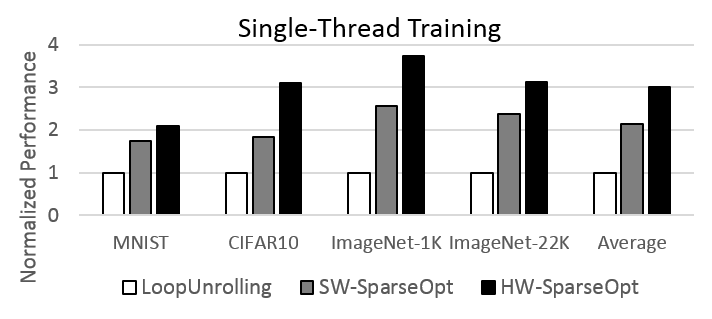
\includegraphics[width=.95\columnwidth]{Figures/computation_sparsity_speedup.png}
\caption{Computation sparsity optimization speedups.}
 \label{fig:computation_sparsity_speedup}
 \end{figure}

To understand why {\it HW-SparseOpt} outperforms {\it SW-SparseOpt}, we examine the impact of computation sparsity optimizations on the training phases.  Figure~\ref{fig:training_breakdown} reports the processing time for a single input in the {\it LoopUnrolling}, {\it SW-SparseOpt}, and {\it HW-SparseOpt} versions of the training phases.  The {\it LoopUnrolling} results show that the three phases contribute roughly equally to overall training time in the baseline case.  Recall that {\it SW-SparseOpt} is used only on back-propagation and weight updates, but not feed-forward evalution, because of the cost/benefit tradeoff.   Thus, {\it SW-SparseOpt} is limited to about \(\frac{2}{3}\) of training execution, where it provides significant overhead reduction (up to $10X$ for ImageNet-1K) because of high computation sparsity in back-propagation and weight updates (Figures~\ref{fig:cifar-10_compute_sparsity}(b) \& ~\ref{fig:cifar-10_compute_sparsity}(c)).   In comparison, {\it HW-SparseOpt} achieves similar overhead reductions for back-propagation and weight updates, and can also be applied to feed-forward execution.  However,  {\it HW-SparseOpt}  achieves much lower overhead reduction in feed-forward evaluation  (at most $1.5X$ for ImageNet-1K) because of lower levels of computation sparsity (~\ref{fig:cifar-10_compute_sparsity}(a)).  Nevertheless, {\it HW-SparseOpt} is overall better than {\it SW-SparseOpt} because feed-forward evaluation becomes the bottleneck after optimizing the other phases, and so that even modest improvements are noticeable in the overall training time.

 \begin{figure*}
 \centering
 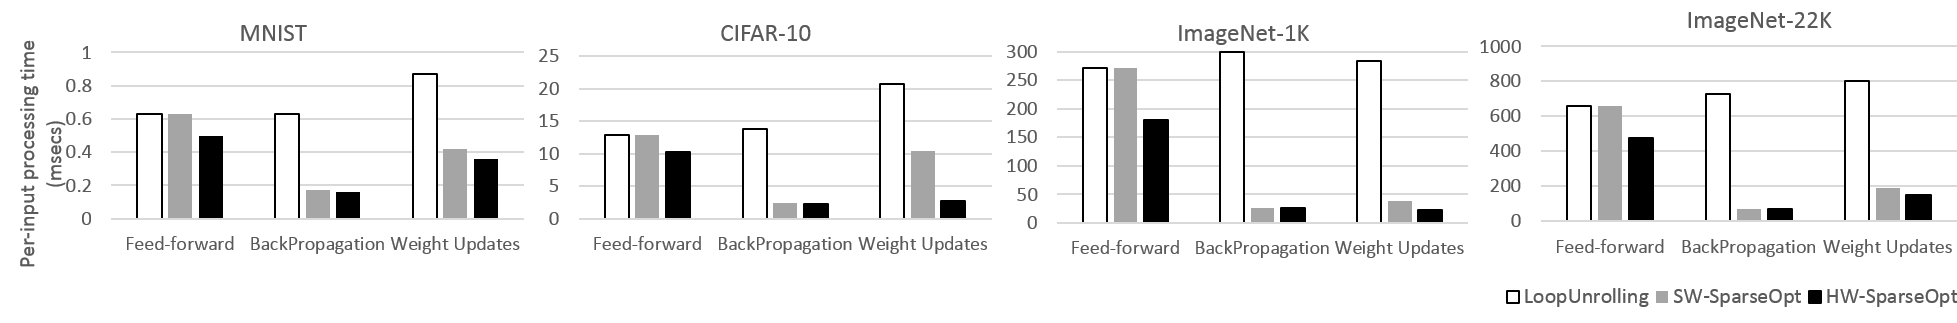
\includegraphics[height=0.75in, width=1.95\columnwidth]{Figures/training_time_breakdown.png}
\caption{Impact of computation sparsity optimizations on training phases.}
 \label{fig:training_breakdown}
 \end{figure*}


\subsubsection{Multi-threaded Performance}
Next we consider the impact of computation sparsity optimizations on multi-threaded training scalability.  Figure~\ref{fig:compute_scaling} shows the normalized training performance as we scale the number of training threads up to $16$, where the baseline performance is the single-threaded {\it LoopUnrolling}.   We make three observations from these results.  First, we see that the benefits of exploiting computation sparsity is sustained and even grows with multi-threading.  Second, we see that larger models (ImageNet-1K and ImageNet-22K) which scale poorly due to their large working sets benefit more from computation sparsity optimizations than relatively smaller models (MNIST and CIFAR-10) because of the reduced pressure placed on shared cache capacity and bandwidth by multi-threading.  Third, we see that {\it HW-SparseOpt} continues to outperform {\it SW-SparseOpt} with multi-threading. 

 \begin{figure*}
 \centering
 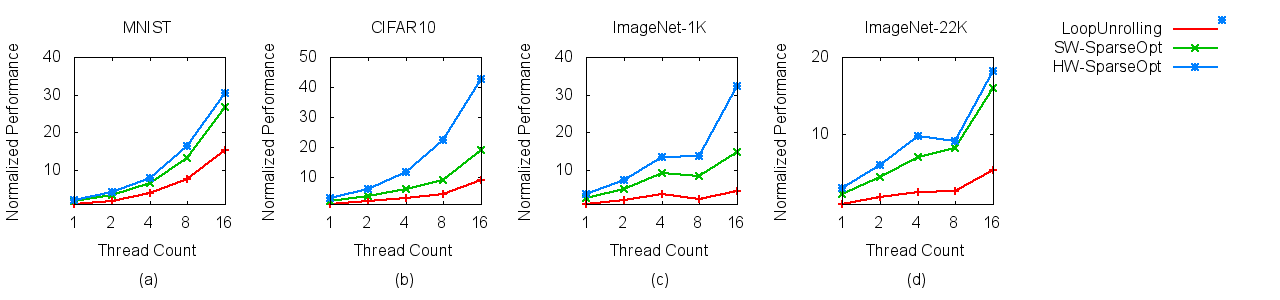
\includegraphics[width=1.95\columnwidth]{Figures/compute_scaling.png}
\caption{Impact of computation sparsity optimization on training scalability.}
 \label{fig:compute_scaling}
 \end{figure*}


\subsection{Data Sparsity Optimizations}
\label{subsec:data_sparsity_perf}

\subsubsection{Multi-threaded Performance}
\label{subsec:perf_multi_thread}

Here we show improved scalability by reducing the cache capacity and bandwidth pressure. 


\subsubsection{Model-parallelism Performance}
\label{subsec:perf_model_parallel}

Here we show improved scalability of model-parallelism because the reduced cache capacity and bandwidth pressure allows bigger models to fit on a machine. 
